%-----------------------------------------------------------------------------------------------
\documentclass[addpoints, 11pt]{exam}
\usepackage[margin=.75in]{geometry}
\usepackage{etex}
\usepackage{graphicx}
\usepackage{amssymb}
\usepackage[fleqn]{amsmath}
\usepackage{nccmath}
\usepackage{cases}
\usepackage{hyperref}
\usepackage{multicol}
\usepackage{tikz}
\usepackage{pgfplots}
\usepackage{float}
\usetikzlibrary{patterns}
\usepackage{pstricks-add}
%\usepackage{pst-func}
%\usepackage{pst-plot}
%\usepackage{pst-spectra}
\usepackage{multido}
\usepackage{lastpage}
\usepackage{ulem}
\usepackage[outside]{coordsys}
\usepackage{float}
\usetikzlibrary{pgfplots.statistics}
\usetikzlibrary{positioning, shapes.geometric}
\pgfplotsset{compat=1.18}
%-------------------------------------------------------------------------------------------------
\setlength{\columnsep}{.5cm}
\setlength{\columnseprule}{1pt}
\newcommand{\ds}{\displaystyle}
\newcommand{\work}{{\bf{No Work $\Leftrightarrow$ No Points }}}
\newcommand{\neat}{{\bf{Use Pencil Only $\Leftrightarrow$ Be Neat \& Organized }}}
\newcommand{\answer}{\large\bf Ans: \underline{\hspace{1.5in}}}
\newcommand{\la}{\lambda}
\newcommand{\zz}{\mathbb{Z}}
\newcommand{\rr}{\mathbb{R}}
\newcommand{\nn}{\mathbb{N}}
\newcommand{\qq}{\mathbb{Q}}
\newcommand{\cc}{\mathbb{C}}
\newcommand{\cyclic}[1]{\langle #1 \rangle}
\newcommand{\lcm}{{\rm{lcm}}}
\renewcommand{\solutiontitle}{\noindent\textbf{Answer:}\par\noindent}
%------------------------------------------------------------------------------------------------
\begin{document}
%------------------------------------------------------------------------------------------------
\cfoot{UCLA: C. Johnson}
%	\rfoot{Total Points: \numpoints}
\rfoot{Page \thepage\ of \pageref{LastPage}}
%------------------------------------------------------------------------------------------------
\begin{center}
	\fbox{%
		\parbox{1\linewidth}{%
			\noindent \Large\bfseries \\[.05in] Math 142: Modeling{\hspace{1.2in}{\Large\bfseries Name:{\hrulefill}}\\[.2cm]
				\noindent \Large\bfseries Homework \# 1 \hspace{2.8in}{Due:} Friday Oct6
			}\\[.025in]
		}%
	}
\end{center}
\addpoints


\vspace{.25cm}


%------------------------------------------------------------------------------------------------
\noindent  {\bf Directions} Complete the exercises. Your solutions to the exercises should be submitted to Gradescope before the indicated due date above. Please follow rules regarding Gradescope submission as described in the syllabus. \\


\noindent{\bf References} Except for the help of the instructor or TAs and the class textbooks and notes, if you use any resources, for example, a book, a website, or you discussed with your friends, please acknowledge them in this References section. 
\begin{itemize}
	\item I discussed Problem ?? with STUDENT A, STUDENT B, $\ldots$
	\item I used BOOK/WEBSITE to help me do Problem ??.
\end{itemize}
\vspace{.05cm}
%\hrule
%----------------------------------------------------------------------------------------------  
\noindent {\bf Exercises}
%\begin{multicols*}{2}
\begin{questions}
	
%----------------------------------------------------------------------------------------------  
\question  Review of linear algebra and calculus
\begin{parts}
\part Find the eigenvalues of the matrix
$$
A=\left(\begin{array}{rr}
	1 & -3 \\
	-3 & 1
\end{array}\right)
$$\\

\textbf{Solution:} We find $\lambda_1,\lambda_2$ s.t $\det(A-\lambda I)=0$. Solving the quadratic ${(1-\lambda)}^2-9=0$, we obtain $\lambda_1=-2,\lambda_2=4$.\\
\part It will often be useful to know whether a particular matrix has an eigenvalue bigger than 1. Without explicitly calculating its eigenvalues, show that the matrix
$$
B=\left(\begin{array}{rrr}
	1 & 3 & 1 \\
	-3 & 0 & 1 \\
	0 & 1 & 6
\end{array}\right)
$$
has one eigenvalue that is larger than 1 . Hint: start by calculating $\operatorname{det}(B-I)$. Then explain why $\operatorname{det}(B-\lambda I)$ is negative for sufficiently large values of $\lambda$. Finally explain then why $\operatorname{det}(B-\lambda I)$ must be go through zero for some $\lambda>1$.\\

\textbf{Solution:} WTS by the intermediate value theorem, there exists a $\lambda>1$ s.t $\det(B-\lambda I)=0$.\\
$\det(B-I)=0(-6)-(-3)(14)+0(4)=42$\\
Let $f(t):=\det(B-tI)$ which is a cubic polynomial, a continuous function.
By Cramer's rule, the only contribution to the cubic term comes from 
$(1-t)\begin{vmatrix}
	-t && 1\\
	1 && 6-t\\
\end{vmatrix}$.
It follows that the constant coefficient of the cubic term of the function $f(t)$ is $-1$, and because the rate of growth of the cubic term dominates the lower order terms, $f(t)<0$ for sufficiently large enough values of $t$.
Thus, because $f(t)<0<f(1)$ for sufficiently large $t$, the $IVT$ states there exists some $1<\lambda<t$ s.t $f(\lambda)=\det(B-\lambda I)=0$
Hence, $B$ has an eigenvalue greater than $1$.
\part The Michaelis-Menten formula is often used as a model for how the rate of a chemical reaction depends on the amount of chemical, $x$ that is reacting. According to the formula the rate of the reaction is:
$$
r(x)=\frac{k x}{x+a}
$$
where $k$ and $a$ are both positive constants, and the amount of chemical, $x \geq 0$. We will use calculus tools to draw the graph of the function $r(x)$.
\begin{parts}
\part Show that $r^{\prime}(x)>0$. That is, $r$ is an increasing function.\\
\textbf{Solution:}
$$
r'(x)=\frac{d}{dx}r(x)=k\frac{(x+a)-x}{{(x+a)}^2}=k\frac{a}{{(x+a)}^2}>0\\ 
$$
for all $x\ge0$ because the square of a number is always positive and $k$ and $a$ are both positive constants.
\part Carefully explaining your reasoning, show that $r(x) \rightarrow k$ as $x \rightarrow \infty$.\\
\textbf{Solution:}
$$
\displaystyle \lim_{x\rightarrow\infty}r(x)=k\frac{x}{x+a}=k\lim_{x\rightarrow\infty}\frac{x}{x+a}=k\frac{1}{1}=k
$$
by infinity over infinity L'H rule.
\part Show that $r^{\prime \prime}(x)<0$. What does this mean for the shape of the graph of $r(x)$ ?\\
\textbf{Solution:}
$$
r''(x)=\frac{d}{dx}r'(x)=k\frac{-2a}{{(x+a)}^3}<0
$$
because ${(x+a)}^3>0$ for $x\ge0$ (multiplying positive numbers yields a positive product) and $k$ and $a$ are both positive constants, so $k\frac{-2a}{{(x+a)}^3}<0$.\\
Thus, we can expect the graph of $r(x)$ to assymptotically approach $k$ from below with an $x$ and $y$ intercept of $0$. We can also say that the function is always increasing, but the rate at which it is increasing is decreasing (concave down).
\part Putting all of your information together, draw a sketch showing the shape of the graph of $r(x)$ as a function of $x$.\\
\textbf{Solution:}
\begin{figure}[H]
	\centering
	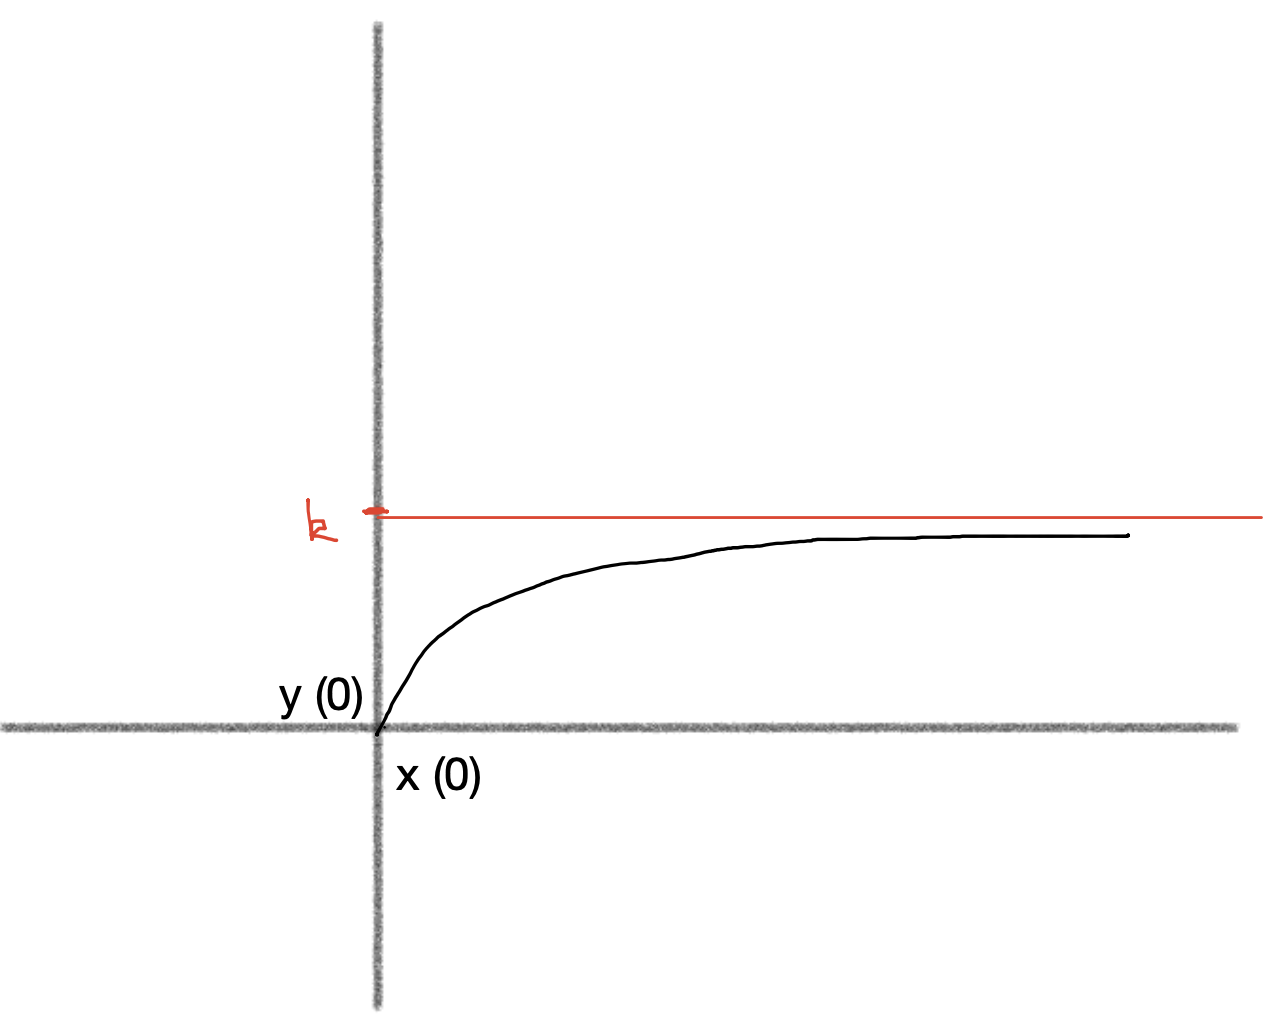
\includegraphics[scale=0.2]{Screenshot 2023-09-28 at 1.07.36 PM.png}
\end{figure}
\end{parts}
\newpage
\item We will meet compartment models, which show up as models for how matter or energy moves through systems. As part of the modeling, we will derive a formula for the concentration of a solute in a tank, that has inflows and outflows. We will find that the concentration of solute, $c(t)$, evolves according to an equation:
$$
\frac{d c}{d t}=c_{\infty}-c
$$
where $c_{\infty}$ will be the constant concentration of solute in the tank inflow. (You don't need to derive this equation). Solve this differential equation, assuming that $c(0)=c_0$ (the unknown constants $c_0$ and $c_{\infty}$ will appear in your answer). Then, by analyzing your solution, show that, no matter what the value of $c_0, c(t) \rightarrow c_{\infty}$ as $t \rightarrow \infty$\\
\textbf{Solution:}
$$
\frac{d c}{d t}=c_{\infty}-c\Rightarrow \frac{d c}{d t}+c=c_{\infty}\Rightarrow c(t)=\frac{\int e^{\int 1dt}c_{\infty}dt+c}{e^{\int 1 dt}}=c_\infty+ce^{-t}=c_\infty+(c_0-c_\infty)e^{-t}
$$
given the initial condition of $c(0)=c_0$\\
Since $\lim_{t\rightarrow\infty}e^{-t}=0$,\\
$\displaystyle \Rightarrow \lim_{t\rightarrow\infty}c(t)=\lim_{t\rightarrow\infty}c_\infty+(c_0-c_\infty)e^{-t}=c_\infty+(c_0-c_\infty)\lim_{t\rightarrow\infty}e^{-t}=c_\infty+0=c_\infty$
\end{parts}
%----------------------------------------------------------------------------------------------   
\question Our model for population growth started from a word equation for how population size changes from time $k$ to time $k + 1$; this question will give you some practice on how to write down these word equations:, both for population growth and for other systems that can be modeled using recurrence equations.\\

You are building a mathematical model for the number of students attending UCLA. Write a word equation relating to the population $N_k$ in one quarter to the population $N_{k+1}$ in the next quarter. Your {\bf word} equation should include the following terms. 
\begin{itemize}
	\item $\#$ students admitted to the university that quarter
	\item $\#$ students that completed their degree (graduated)
	\item $\#$ students that returned from a break
	\item $\#$ students that are taking the quarter off
\end{itemize}
\textbf{Solution:} \\
$\begin{pmatrix}
	\text{\# students}\\
	\text{@ quarter }k+1
\end{pmatrix}$ =
$\begin{pmatrix}
	\text{\# students}\\
	\text{@ quarter }k
\end{pmatrix}$ +
$\begin{pmatrix}
	\text{\# returned from break}\\
	\text{@ quarter }k
\end{pmatrix}$ +
$\begin{pmatrix}
	\text{\# admitted}\\
	\text{@ quarter }k
\end{pmatrix}$ -
$\begin{pmatrix}
	\text{\# quarter off}\\
	\text{@ quarter }k
\end{pmatrix}$ - 
$\begin{pmatrix}
	\text{\# completed degree}\\
	\text{@ quarter }k
\end{pmatrix}$

%$N_{k+1}=N_k+\{\text{$\#$ students admitted to the university that quarter}-\text{$\#$ students that completed their degree}\}+\\\{\text{$\#$ students that returned from a break}-\text{$\#$ students that are taking the quarter off}\}$
%----------------------------------------------------------------------------------------------   
\question You are trying to build a mathematical model for the population of red-wolves in North Carolina. Red wolves are a critically endangered species, once found throughout the southeastern United States but now found mainly in a single North Carolina wildlife reserve. The data in this question come from a report published by the U.S. Fish and Wildlife Service in 2007: "Red Wolf (Canis rufus) 5-Year Status Review: Summary and Evaluation".
\begin{parts}
\part If the population size $t$-years after the start of a study on red wolf numbers is $N_t$, start by writing down a word equation so that $N_{t+1}$ can be predicted from $N_t$ :
$$N_{t+1}=N_t+ \left(\text{ number of pups born }\right)-\left(\text{ number of wolves that die}\right)$$
We will start by deriving expressions for the birth and death rates.
\begin{parts}
\part It is possible to count the number of pups born in given year. A subset of these data (taken from the US Fish and Wildlife Service report) is given in the following table:

\begin{tabular}{|c|c|c|}
	\hline Year & $N_t$ & Number of pups born \\
	\hline \hline 1990 & 18 & 3 \\
	\hline 1993 & 44 & 16 \\
	\hline 1996 & 70 & 16 \\
	\hline 1999 & 126 & 37 \\
	\hline 2002 & 123 & 33 \\
	\hline 2005 & 115 & 41 \\
	\hline
\end{tabular}

Plot the number of pups against the population size $N_t$. Show that the data are consistent with the following formula for the number of pups born in one year:
Number of pups born in one year $=0.28 N_t$\\
\textbf{Solution:} \\
\begin{figure}[H]
	\centering
	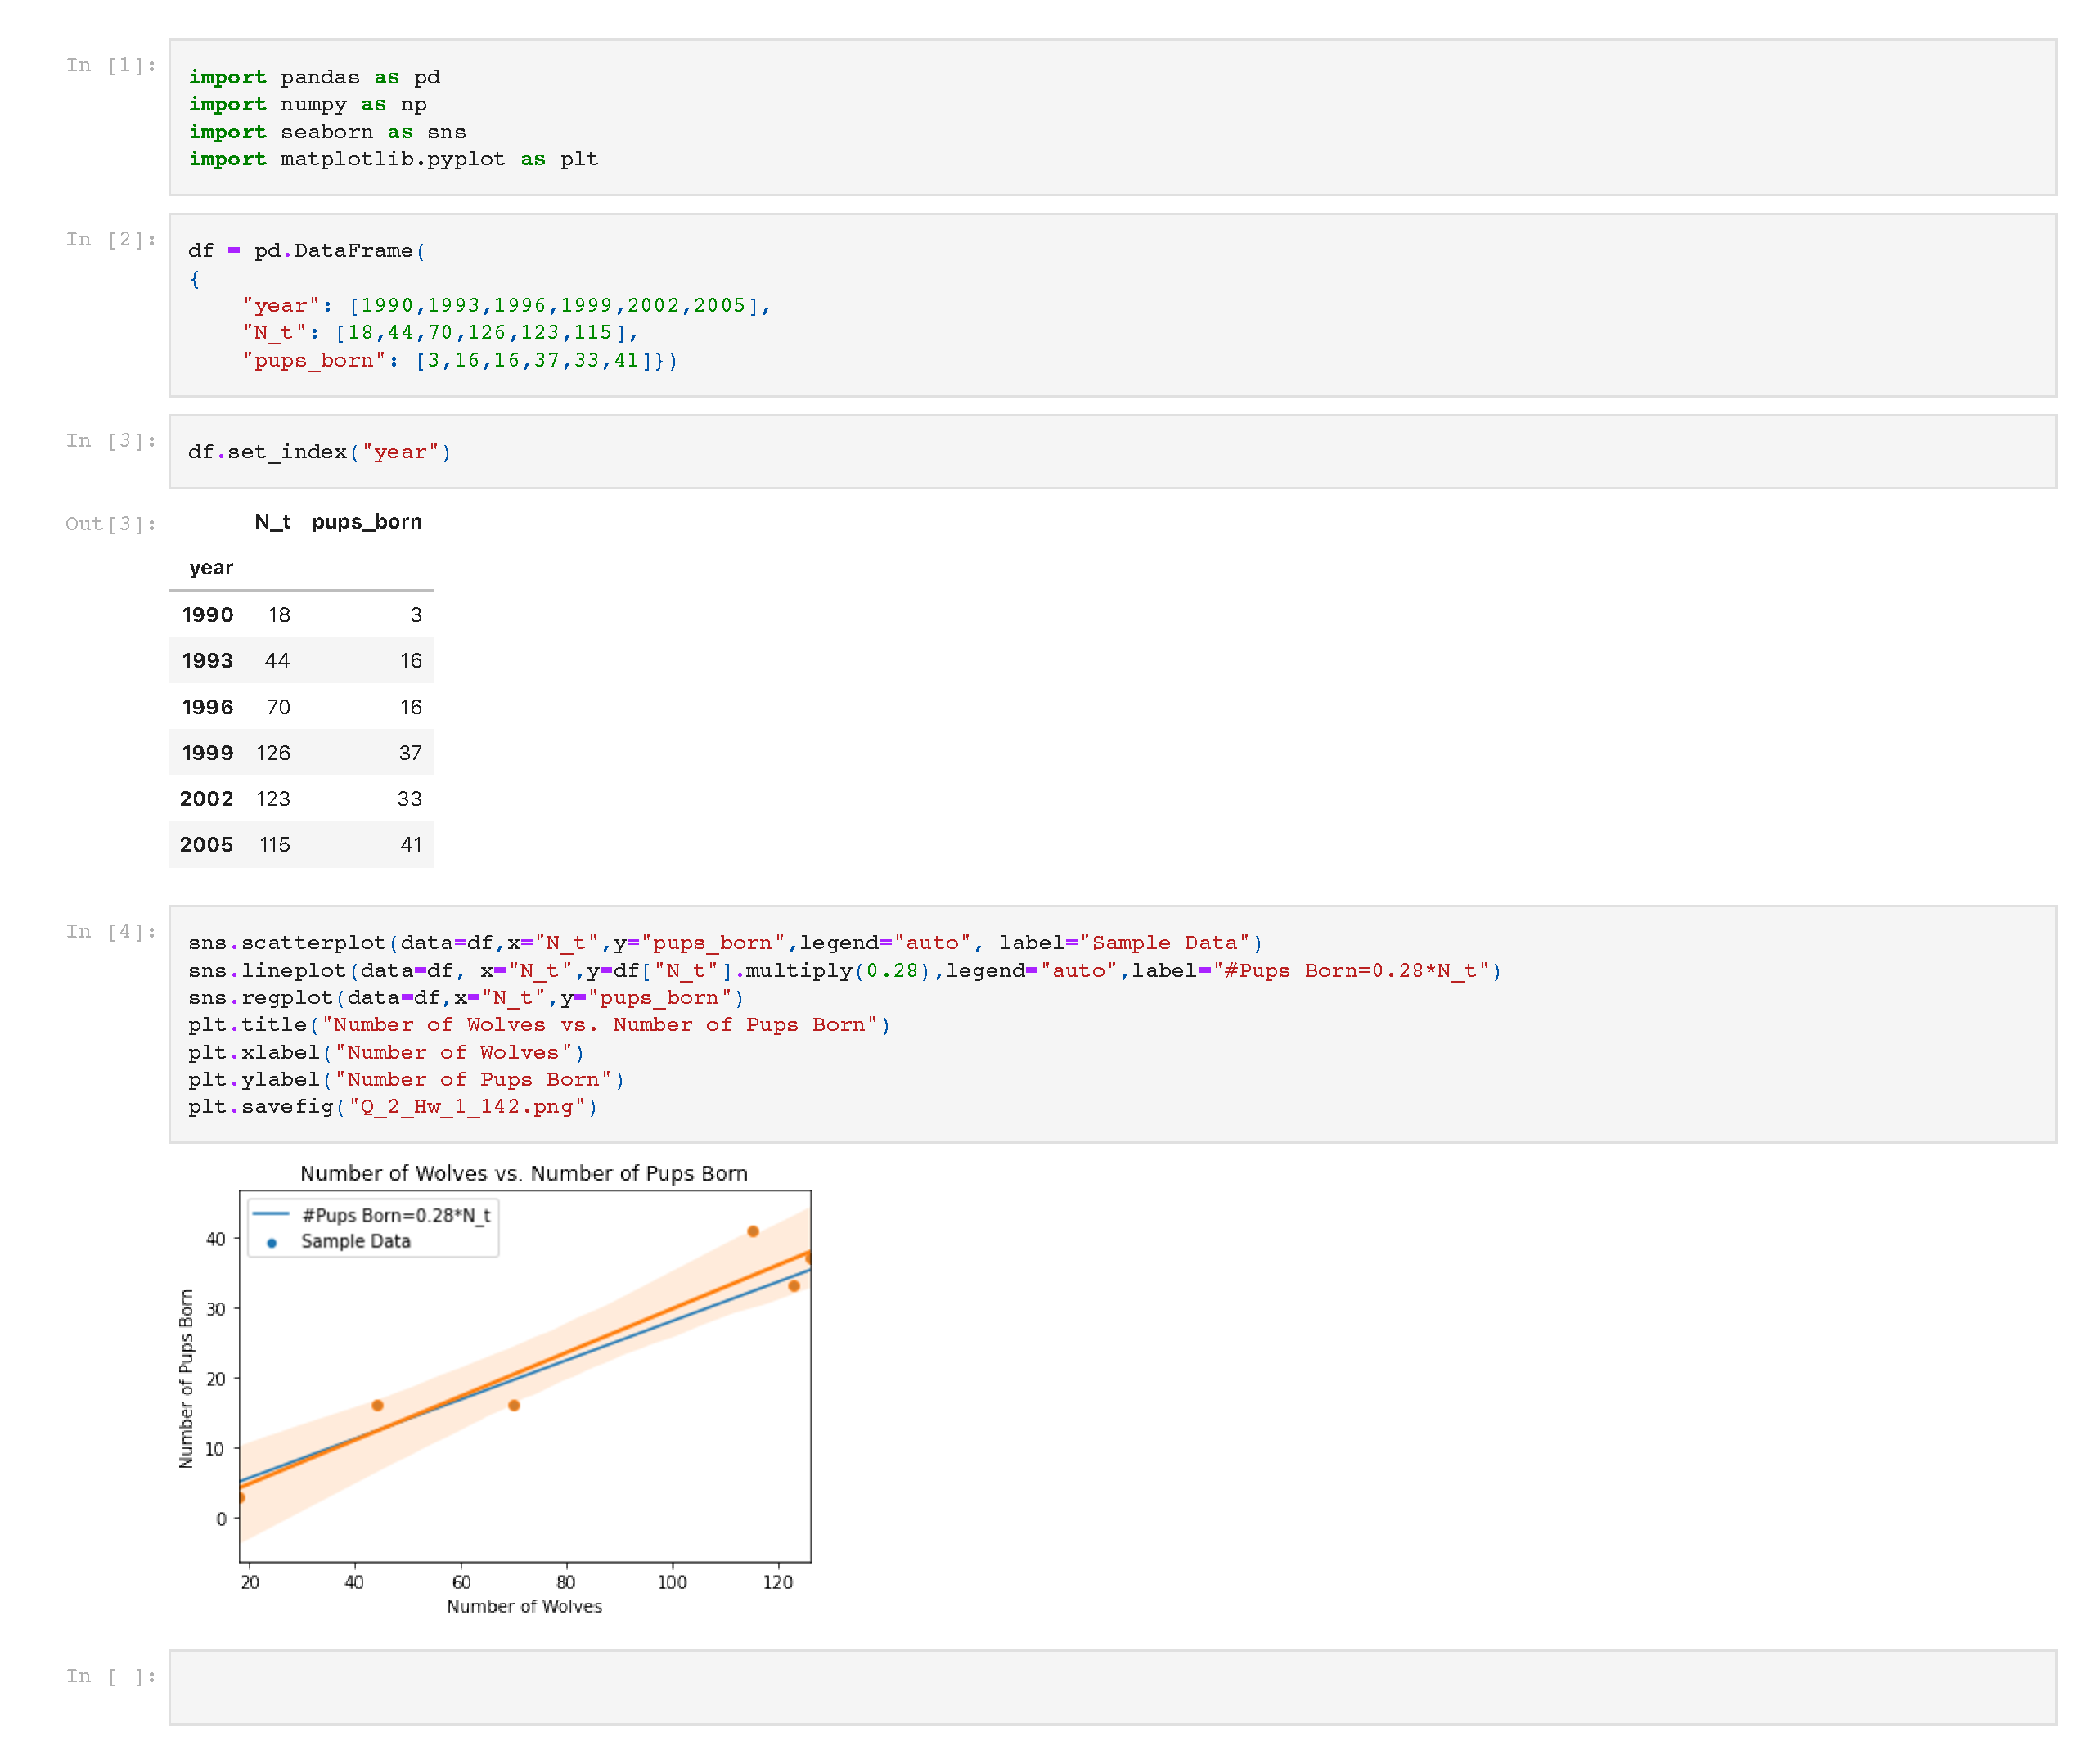
\includegraphics[scale=0.4]{Math_142_HW_1.pdf}
\end{figure}
The sample regression line doesn't differ significantly from the proposed linear relationship between the number of wolves and number of pups born, so it would not be unreasonable to assume that the sample data comes from a population that is consistent with the formula Number of pups born in one year$=0.28N_t$.
\part Conservationists also measure the number of red wolf deaths in each year: the main causes of death are being killed by hunters and ranchers, or by being struck by vehicles. They estimate that in one year $22 \%$ of red wolves are killed. Write down recurrence relation for the population size $N_t$ including both birth and death rates.\\
\textbf{Solution:} \\
$
N_{k+1}=N_k+b\Delta t N_k-m\Delta t N_k\\
\Delta t=\text{1 year}, b=0.28,m=0.22\\
N_{t+1}=N_t+0.28N_t-0.22N_t=(1.06)N_t
$
\end{parts}
\part Assuming that the current population size is $N_0=130$ wolves, use your formula from (a) to predict the population size $N_t$ for the next 5 years (that is, calculate $N_1, N_2, \ldots, N_5$ ).\\
\textbf{Solution:} \\
$
N_1=(1.06)N_0=137.8\\
N_2=(1.06)N_1=146.1\\
N_3=(1.06)N_2=154.8\\
N_4=(1.06)N_3=164.1\\
N_5=(1.06)N_4=174.0
$
\part The current conservation goal for the wild red wolf population is to reach 220 individuals. When, according to your model, will that population size be reached?\\
\textbf{Solution:} \\
$
N_t={(1.06)}^t N_0\\
\log(N_t)=t\log(1.06)+\log(N_0)\\
\Rightarrow t=\frac{\log(\frac{N_t}{N_0})}{\log(1.06)}\\
N_t=220,N_0=130\\
\Rightarrow  t=\frac{\log(\frac{220}{130})}{\log(1.06)}=9.0287\\
$
The population will have reached 220 individuals after 10 $\mathit{ (9.0287)}$ years.
%	\part In addition to the wild red wolf population there is a captive breading population. One strategy is to introduce captive bred wolves into the wild. Suppose that 10 captive bread wolves are added to the wild population each year. Unfortunately, captive bred wolves do not readily integrate into existing packs, and are less effective hunters than wild-born wolves. As a result $43 \%$ of introduced wolves die each year. To model the effect of introducing wolves, we must keep track of both the number of wild-born wolves, $N_t$ and the number of wolves that are introduced $I_t$.
%	\begin{parts}
%	\part Explain why:
%	$$
%	\begin{aligned}
%		N_{t+1} &=1.06 N_t+0.28 I_t \\
%		I_{t+1} &=10+0.57 I_t
%	\end{aligned}
%	$$
%	(explain what each term in the equations represents). Also explain why the total number of wild red wolves is given by $N_t+I_t$
%	\part Calculate $N_t$ and $I_t$ for $t=0,1,2,3,4,5$, assuming that $N_0=130$ and $I_0=0$. Then, using Matlab, or by some other means, calculate when the total number of wild red wolves will reach the target population size of 220 .
%	\part Make a plot of how the population size grows as a function of $t$. Show that the growth is eventually exponential.
%	\end{parts}
\end{parts}
%---------------------------------------------------------------------------------------------- 
\question You are trying to use your population growth model from class to model the growth of a population of yeast cells, and to compare to real data. The real data we will use is from a paper by Carlson. You should start by downloading the data from the BioQuest website: \href{https://bioquest.org/numberscount/data-details/?product_id=31395}{Bioquest Data}
The data consists of a count of yeast cells (the count is measured in terms of millions of cells per ml of the growth medium), as a function of time.
\begin{parts}
\part Show by plotting the data for population size against time that the population size in Carlson's experiment that the population does not grow exponentially (or at least, does not grow exponentially over the entire time covered by the experiment). We discussed, in class, that populations can not grow exponentially indefinitely because cells compete for resources.
\begin{figure}[H]
	\centering
	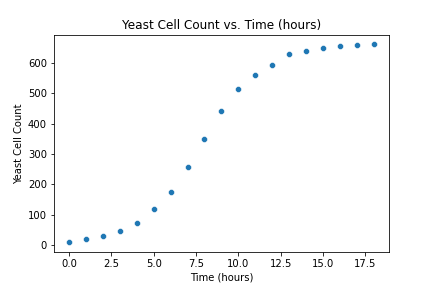
\includegraphics{Q_4_Hw_1_142_a.png}
\end{figure}
\part In fact, in the first few hours of the experiment, the population growth is approximately exponential. Explain how to plot your data in a way that shows that for early times there is exponential growth, and estimate the reproductive rate associated with that exponential growth.
\begin{figure}[H]
	\centering
	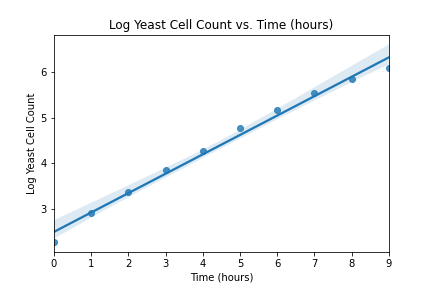
\includegraphics{Q_4_Hw_1_142_b.png}
\end{figure}
We can plot the $\log$ of the Yeast Cell Count against Time (hours). If there exists a linear relationship between the transformed variables for the first few hours $(t<10)$, then the population growth is approximately exponential.\\
\begin{figure}[H]
	\centering
	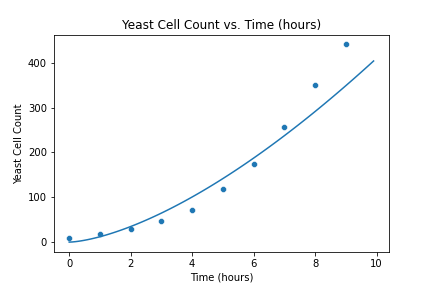
\includegraphics{Q_4_Hw_1_142_c.png}
\end{figure}
$N_{k+1}\approx(1.5328)N_k\Rightarrow R_0 \approx0.5328$
\part Let's consider how we might modify our model to account for the fact that the reproductive rate is not a constant. Suppose that the reproductive rate $R_0$ depends on the population size. That is $R_0 \equiv R_0\left(N_k\right)$. So our model for population growth is:
$$
N_{k+1}=\left(1+R_0\left(N_k\right) \Delta t\right) N_k
$$
How can we find the function $R_0\left(N_k\right)$ ? Rearrange our equation in the form:
$$
\frac{N_{k+1}-N_k}{N_k \Delta t}=R_0\left(N_k\right)
$$
the left hand side of the equation is the relative increase in population size between censuses (divided by time). For the Carlson data plot this quantity against $N_k$.
\begin{figure}[H]
	\centering
	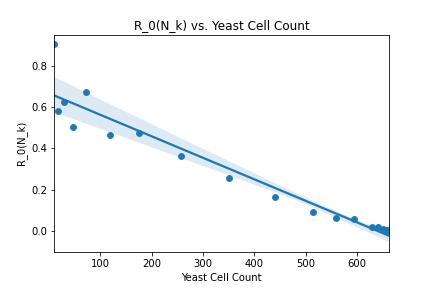
\includegraphics{Q_4_Hw_1_142_d.png}
\end{figure}
\part Some researchers have argued that the correct model for the growing population is $$R_0\left(N_k\right)= r\left(1-\frac{N_k}{K}\right),$$ where $r$ and $K$ are positive constants. This model is known as the logistic growth model. Do you think this model is consistent with your graph from (c)? Briefly justify your answer.\\
The graph in part (c) follows the same inverse relationship as the proposed formula, and there is a strong correlation between the two variables. 
\part The positive constant $K$ is usually called the carrying capacity of the population. Thinking about the new model, can you briefly describe what $K$ represents?\\
The carrying capacity represents the max number of organisms that an environment/ecosystem can support. This can occur when environmental pressures caause the net reproduction rate to go to $0$.
\end{parts}
\begin{figure}[H]
	\centering
	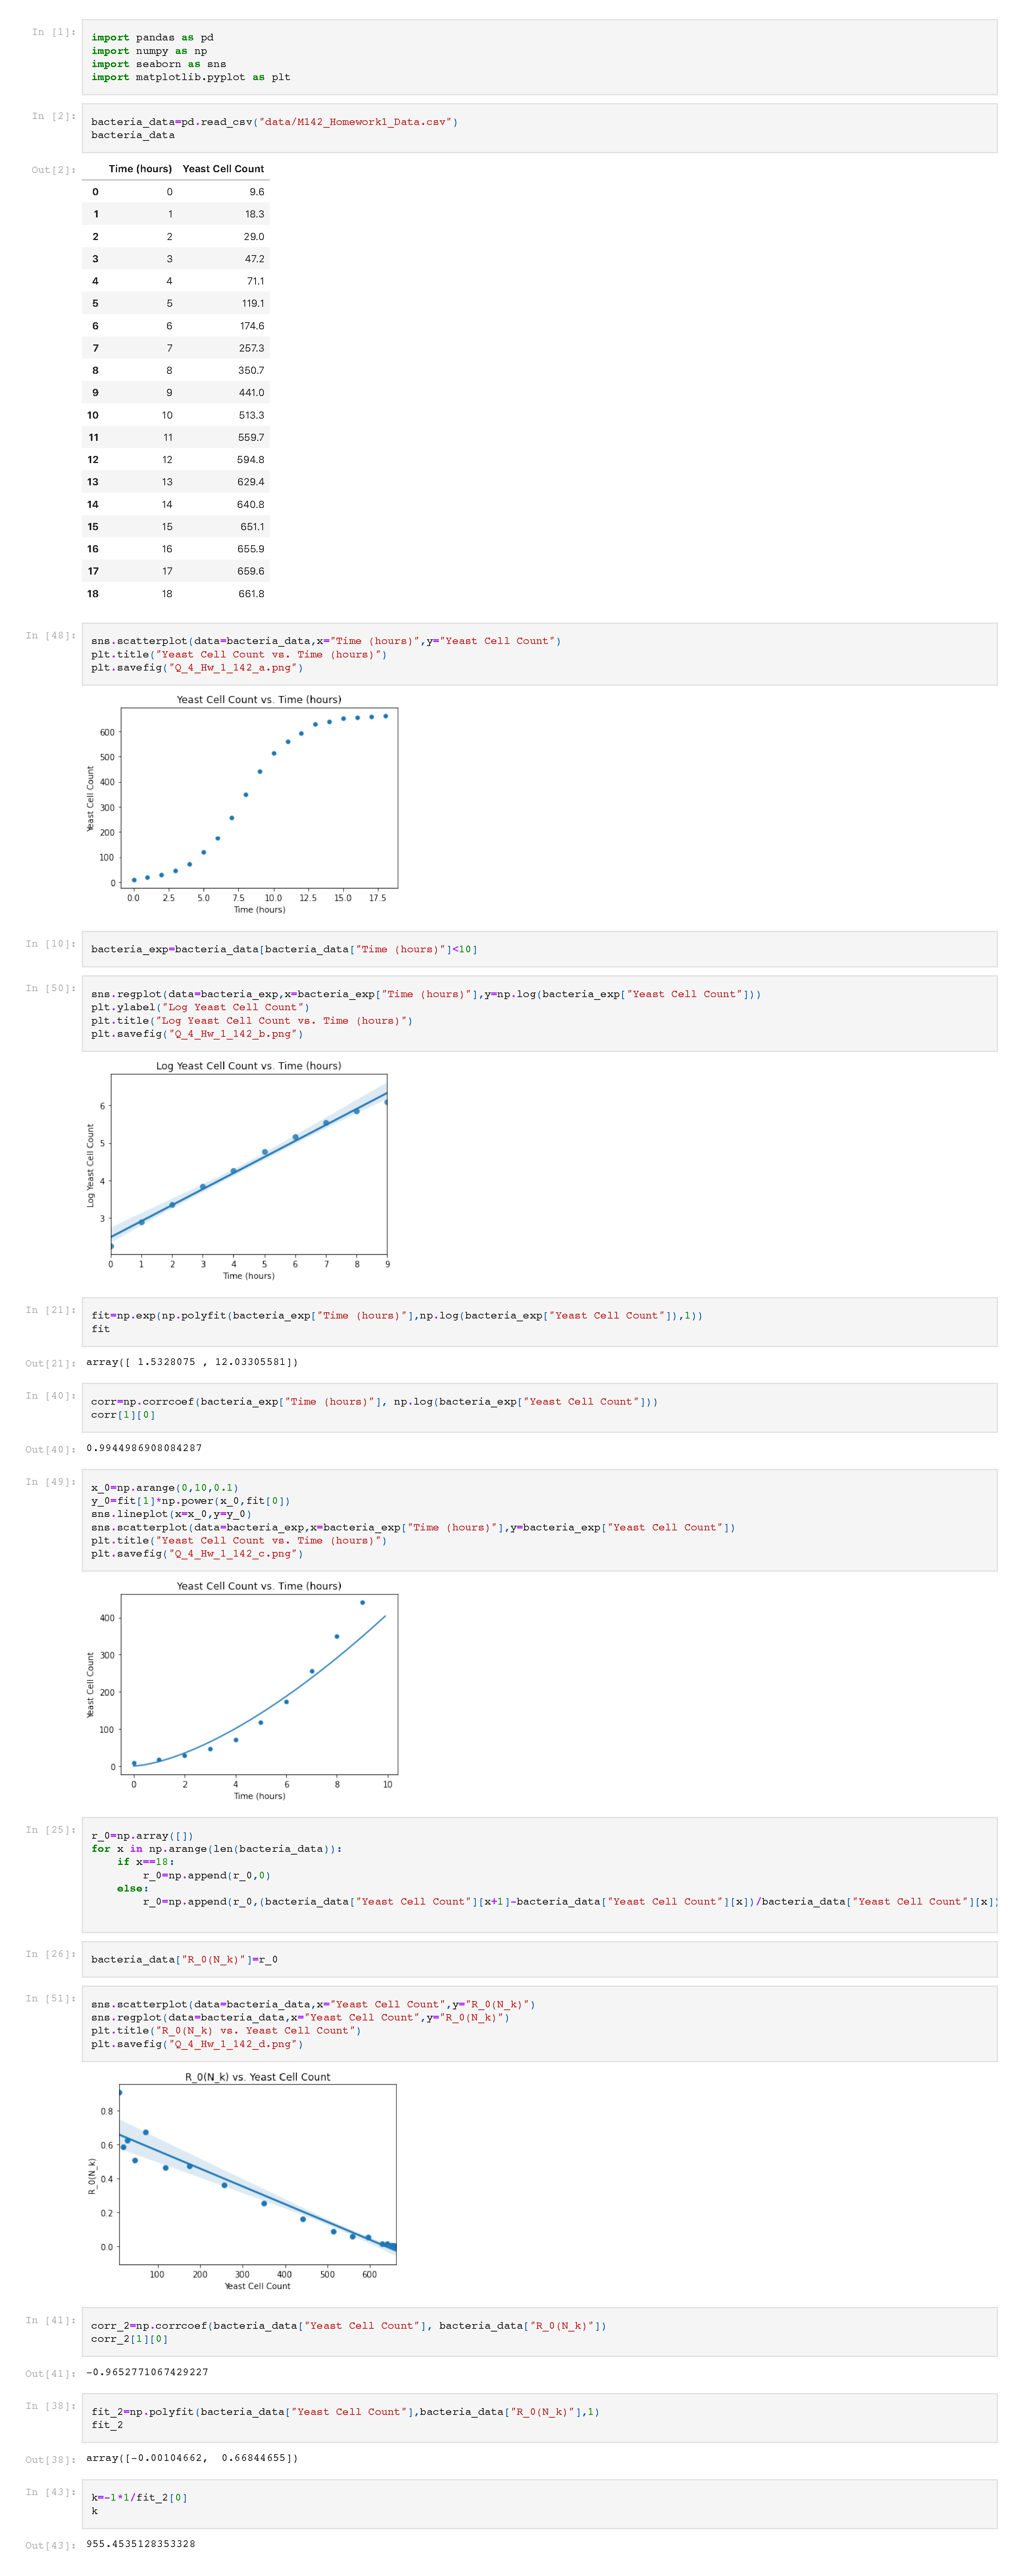
\includegraphics[scale=0.22]{Math_142_HW_1-Copy1.pdf}
\end{figure}
%----------------------------------------------------------------------------------------------


\end{questions}
%\end{multicols*}
\end{document}